\documentclass[a4paper, twoside, 11pt]{book}
\usepackage[utf8]{inputenc}
\usepackage{geometry}
\usepackage{graphicx}
\usepackage{setspace}
\usepackage[inline]{enumitem}
\usepackage{amsmath}
\usepackage{amsthm}
%\usepackage{hyperref}


\newtheorem{remark}{Remark}
\newtheorem{observation}{Observation}
\newtheorem{note}{Note}
\newtheorem{theorem}{Theorem}

\pagestyle{plain}%used to clear header with chapter and section titles

\begin{document}

\frontmatter
\begin{titlepage}
\newgeometry{margin=3.5cm}

\begin{center}


\includegraphics[width=9cm]{Frontmatter/Cover/logo-unitn.jpg}\\[0.4cm]

{\LARGE Department of Physics}\\[4.5cm]

{\Large Bachelor's Degree in Physics}\\[0.5cm]

{\Large Final thesis}\\[0.5cm]

% Title
\rule{\linewidth}{0.2mm} \\[0.5cm]

{ \huge \bfseries Bell's theorem without inequalities \\[0.5cm] }

\rule{\linewidth}{0.2mm} \\[2cm]

% Author and supervisor
\begin{minipage}{0.4\textwidth}
\begin{flushleft} \large
\emph{Supervisor:} \\[0.25cm]
Prof. Franco Dalfovo
\end{flushleft}
\end{minipage}
\begin{minipage}{0.4\textwidth}
\begin{flushright} \large
\emph{Graduand:}\\[0.25cm]
Severino Zeni
\end{flushright}

\end{minipage}

\vfill

% Bottom of the page
{\large A.Y. 2013/2014}

\end{center}

\restoregeometry
\end{titlepage}


\onehalfspacing%sets interline spacing to 1.5 from here onwards, consider doing it with \linespread{}

%\copyrightpage
\chapter*{Preface}
Quantum mechanics describes physical systems by means of a state vector, $| \psi \rangle$. For systems extended in space a description of a portion of the system (located in some space region) cannot in general be given without taking into account all other constituents of the system (no matter how far these are). This is at the basis of the phenomenon of entanglement.

In 1935 Albert Einstein, Boris Podolsky and Natan Rosen (EPR) realized that entanglement allowed a step further in the discussion on the foundations of quantum mechanics. In particular it allowed them to show that, under reasonable assumptions, $| \psi \rangle$ could not be regarded as a satisfactory description of single physical systems. Under these assumptions, $| \psi \rangle$ could provide at most correct description of statistical ensembles of systems.

The next milestone in the discussion was the contribution by John S. Bell. In 1964 he showed that the premises of the EPR argument lead to an inequality (Bell's inequality) that is violated by statistical predictions of quantum mechanics. This inequality allows experimental tests of the quantum mechanical predictions against those descending from EPR's assumptions. Since the seventies a variety of such tests have been made with no one being able to disprove quantum mechanics.

This thesis will be concerned with some elements of this debate. In Chapter \ref{chap:epr} we will present the EPR argument. Bell's reasoning will not be illustrated in favor of a more recent result on the same matter that Daniel M. Greenberg, Michael A. Horne and Anton Zeilinger (GHZ) proposed in 1989 (Chapter \ref{chap:ghz-theorem}). Finally, Chapter \ref{chap:ghz-experiments} will be concerned with some of the experimental efforts that have been made towards a test of quantum mechanics following the argument by GHZ.

We will see that the GHZ argument will lead us to conclusions analogous to those obtained by Bell but in a way that doesn't involve inequalities. We will also see, that from an experimental point of view, the argument allows, in principle, to design experiments in which a single run suffices to confirm or disprove quantum mechanics. This is in contrast with experiments that follow Bell's argument where statistical considerations on many runs of the experiment must be done.

\tableofcontents
%\acknowledgments
%\include{Frontmatter/notation}

%mainmatter
\mainmatter
\chapter{The EPR program}

The first section of this chapter will concern the argument brought foreward by Einstein, Podolsky and Rosen in their article \cite{PhysRev.47.777}, in particular the adaptation of the argument proposed by Bohm in \cite{bohm1951quantum} will be treated (see also \cite{PhysRev.108.1070}).
It will be shown that under reasonable assumptions, regarding the locality of physical processes and reality, the quantum description of reality is incomplete (i.e. there exists \textit{elements of physical reality} for which there is no couterpart in the formalism). TO REVISE

In the last section of the chapter some of Bell's contributions on the matter will be presented. In particular...


\section{EPR ``theorem''}

\begin{figure}
  \centering
  \includegraphics[width=0.25\textwidth]{Mainmatter/Chapter1/eprb.png}
  \caption{Bohm's adaptation of EPR's gedankenexperiment. Two spin-1/2 particles  emitted by the source (in the singlet state of spin)...}
  \label{fig:eprb-gedankenexp}
\end{figure}

\subsection*{EPRB gedankenexperiment}

Consider a system composed of two spin-1/2 particles flying off a source in opposite directions as shown in Fig. \ref{fig:eprb-gedankenexp}. Suppose that the two particles are emitted by the source in the state with total spin equal to $0$, that is in the state:
\begin{equation}
  |\Psi\rangle = \frac{1}{\sqrt{2}} \left( |S_z = + 1\rangle_1 |S_z = - 1\rangle_2 - |S_z = - 1\rangle_1 |S_z = + 1\rangle_2 \right)
  \label{eq:singlet-state}
\end{equation}
Once the two particles are far from each other they enter two apparatuses which can measure either $S_x$ or $S_y$ (e.g. two Stern-Gerlach apparatuses with magnetic fields oriented either in the $\hat{\textbf{x}}$ or $\hat{\textbf{y}}$ direction).

Let us see what the prediction of quantum mechanics for such an experiment are, in particular we are interested in the (perfect) correlation between the result of the measurement performed on the particle propagating in the positive $\hat{\textbf{z}}$ direction (which we will call particle A from now on) with that on the particle propagating in the negative $\hat{\textbf{z}}$ direction (particle B).

REPHRASING NEEDED

Suppose that both apparatuses are set to measure $S_x$, to obtain the prediction it is convenient to express the state (\ref{eq:singlet-state}) on a basis of eigenvectors of the $S_x$ observable. It turns out that the state in question takes the same form on any basis of the spin space (see Appendix \ref{app:spin-rotations}), and thus:
\begin{equation*}
  |\Psi\rangle = \frac{1}{\sqrt{2}} \left( |S_x = + 1\rangle_1 |S_x = - 1\rangle_2 - |S_x = - 1\rangle_1 |S_x = + 1\rangle_2 \right)
\end{equation*}
We can see that if the particle propagating in the positive $\hat{\textbf{z}}$ direction is found to have $S_x = + 1$ ($S_x = - 1$) then the other particle will be found to have $S_x = - 1$ ($S_x = + 1$).
We have just said that the state (\ref{eq:singlet-state}) takes the same form on any basis of the spin space, thus if both apparatuses are set to measure $S_y$ we obtain analogous results.

\subsection*{EPR argument}

In the previous paragaph we have only presented some aspects of the quantum mechanical description of systems composed of two spin-1/2 particles. We are now ready to present the EPR argument.
Let us start by listing the assumptions on which the argument rests:
\begin{enumerate}
  %enumerated lists style
  \renewcommand{\theenumi}{\alph{enumi}}
  \renewcommand{\labelenumi}{(\theenumi)}
\item \label{itm:perfect-correlations} \textit{Perfect correlation:} If the spins of the two particles are measured along the same direction, then the two spins will be found (with certainity) to have opposite sign.
\item \label{itm:epr-locality} \textit{Locality:} ``Since at the time of measurement the two systems no longer interact, no real change can take place in the second system in consequence of anything that may be done to the first system.''
\item \label{itm:epr-reality} \textit{Reality:} ``If, without in any way disturbing a system, we can predict with certainity (i.e. with probability equal to unity) the value of a physical quantity, then there exist an element of physical reality corresponding to this physical quantity.'' ADD SOMETHING HERE
\item \label{itm:epr-completeness} \textit{Completeness:} ``Every element of the physical reality must have a counterpart in the [complete] physical theory.''
\end{enumerate}
The first of these assumptions, as we have seen, is a prediction of quantum mechanics. The three latter ones are reasonable propositions about locality, reality and completeness of a physical theory which we have quoted from the original article by Einstein, Podolsky and Rosen \cite{PhysRev.47.777}.

The agrument is then the following:
\begin{enumerate*}
\item Perfect correlations, (\ref{itm:perfect-correlations}), allow us to predict \textit{with certainity} the outcome of a spin component measurement on the particle B by first measuring the same spin component on particle A;
\item Because of locality, (\ref{itm:epr-locality}), the measurement performed on particle A cannot cause a change on particle B.
\item By reality, (\ref{itm:epr-reality}), we can state that the spin component considered is an element of physical reality.
\item We observe that the previous points in the argument hold for both $S_x$ and $S_y$, we must thus admit that the two spin components are both \textit{elements of physical reality} with a definite value. Since there is no state in quantum mechanics in which both spins have definite value we conclude that the quantum mechanicsl description of reality is incomplete.
\end{enumerate*}

THE WORD ENTANGLEMENT NEVER COMES UP

\begin{observation}
The agrument presented here is not the original argument that Einstein, Podolsky and Rosen present in their article \cite{PhysRev.47.777}. The difference being...
\end{observation}

\begin{observation}
  From the results derived in Appendix \ref{app:spin-rotations} it can easily be seen that the argument is more general. In particular it can be shown that the result is not limited to the $\hat{\bftext(x}}$ and $\hat{\bftext(y}}$ components of spin and the argument applies to any component of spin. Hence any component of spin is an \textit{element of physical reality}
\end{observation}

\subsection{Consequences of EPR's result}
The EPR argument 

They don't give a completation

\section{How Bell introduced EPR elements of reality into the formalism}


Bell could derive experimentally testable inequalities... ...we are not going to present here (references)

\chapter{GHZ theorem}
\label{chap:ghz-theorem}
In this chapter we will present an argument to show that the criticism leveled against quantum mechanics by EPR is void, it will be shown that the premises on which EPR's argument rests are incosistent.

The first result of this type is due to John S. Bell and is presented in his work of 1964 \cite{Bell1964}. This thesis will not be concerned with Bell's reasoning but will rather present a more recent argument that leads to the same conclusion. This argument was proposed by Daniel M. Greenberg, Michael A. Horne and Anton Zeilinger in 1989 \cite{ghz1989} (see also \cite{:/content/aapt/journal/ajp/58/12/10.1119/1.16243}).


\section{Summary and formalization of EPR results}

This section serves us to introduce the notation we will use to expose the main matter of this chapter, no new result will be derived here.

In the previous chapter starting from the assumptions of perfect correlation (\ref{itm:epr-perfect-correlation}), completeness (\ref{itm:epr-completeness}), reality (\ref{itm:epr-reality}) and locality (\ref{itm:epr-locality}) we proved the following results:
\begin{enumerate}
  %enumerated lists style
  \renewcommand{\theenumi}{\roman{enumi}}
  \renewcommand{\labelenumi}{(\theenumi)}
\item \label{itm:incompleteness} \textit{Incompleteness:} there are elements of the physical reality that have no couterpart in quantum mechanics.
\item \label{itm:determinism} \textit{Determinism:} the result of a measurement of a spin component (of one of two particles in the state (\ref{eq:singlet-state})) depends on those elements of the physical reality and is predetermined (i.e. no indeterministic process takes place when the measurement is performed).%should i specify spin component of _entangled_ particle?
\end{enumerate}
Result (\ref{itm:incompleteness}) implies that there exists a more complete specification of the physical reality. Let us denote by $\lambda$ this more complete description of a pair of particles compatible with the perfect correlation assumption (\ref{itm:epr-perfect-correlation}), i.e. a description that comprises the elements of physical reality we have found to exist and are ignored by quantum mechanics. Quoting Bell's article \cite{Bell1964}, in which he introduced for the first time this notation: ``It is a matter of indifference ... whether $\lambda$ denotes a single variable or a set, or even a set of functions, and whether the variables are discrete or continuous.'' By (\ref{itm:determinism}) we then deduce (again following Bell \cite{Bell1964}) that the result of a spin component measurement on particle 1, $A$, is a function of $\lambda$, that is:
\begin{equation}
  A = A_i(\lambda)
  \label{eq:results-particle-1}
\end{equation}
where $i = x, y$ denotes the spin component (of particle 1) measured. Analogously, for particle 2, the outcome of a measurement of the $j = x, y$ spin component will be given by the function:
\begin{equation}
 B  = B_j(\lambda).
 \label{eq:results-particle-2}
\end{equation}
%is it clear enough the dependence on the settings of the apparatus?

In writing $A_i(\lambda)$ and $B_j(\lambda)$ this way we have implicitly fullfilled a request that comes from locality, that is: the result of a measurement of a spin component on particle 1 does not depend on the spin component of particle 2 that is measured (i.e. $A$ depends on $i$ only and not on $j$), conversely $B$ only depends on $j$ and not on $i$.%is some better explenation needed here?

\begin{observation}
Working on the objects just presented Bell \cite{Bell1964} could derive a contradiction between the EPR assumptions ((\ref{itm:epr-perfect-correlation}), (\ref{itm:epr-completeness}), (\ref{itm:epr-reality}) and (\ref{itm:epr-locality})) and statistical predictions of quantum mechanics. We will not present his argument here as we will focus on a more recent result on the same matter.
\end{observation}

\begin{observation}
  HERE GOES A COMMENT ABOUT THE WELL DEFINITENESS OF THE FUNCTIONS A, B. THEY ARE WELL DEFINED ``ONLY'' ALMOST EVERYWHERE (see note 14 on ghz article).
\end{observation}


\section{Adaptation of the previous results to systems of three spin-1/2 particles}
\label{sec:adaptation-to-3-particles}
Before moving on to present the main matter of this chapter we need to adapt some of the results obtained so far to systems consisting of more that two particles. In particular we will be concerned with systems of three entangled particles and thus we will limit our attention to this case.%is entangled relevant here?

Consider a system of three spin-1/2 particles in the spin state:
\begin{equation}
  |\chi\rangle = \frac{1}{\sqrt{2}} \left( |+\rangle_1 |+\rangle_2 |+\rangle_3 - |-\rangle_1 |-\rangle_2 |-\rangle_3 \right)
  \label{eq:ghz-state}
\end{equation}
where $|+\rangle_i$ and $|-\rangle_i$ are states of spin up and down along the $\mathbf{\hat{z}}$ direction respectively of particle $i = 1, 2, 3$.
We are interested in the predictions of quantum mechanics for the results of experiments that measure a spin component of each particle, in particular we are interested in the following observables:
\begin{equation}
  \begin{split}
    S_{1x} \times S_{2y} \times S_{3y}\\
    S_{1y} \times S_{2x} \times S_{3y}\\
    S_{1y} \times S_{2y} \times S_{3x}
  \end{split}
  \label{eq:xyy-observables}
\end{equation}
It is easy to show that for all of these quantum mechanics predicts with certainity (i.e. with probability equal to 1) the result $+ 1$ (the proof of this statement is given in Appendix \ref{app:spin-predictions}).

Once again we can observe that the result of a measurement on one of the particles can be predicted with certainity by an appropriate measurement on the other two particles (perfect correlation). If the particles are emmitted at a source and move away from it in different directions, let's say in the $xy$ plane at $120^{\circ}$ form each other, the measurements can be made in places very far from each other. We are thus in a situation analogous to that evisaged by EPR for their argument and the assumptions (\ref{itm:epr-perfect-correlation}), (\ref{itm:epr-completeness}), (\ref{itm:epr-reality}) and (\ref{itm:epr-locality}) can now be written in the form:%is it really just a form issue?

\begin{enumerate}[label=(\alph*$'$)]
  %enumerated lists style
\item \label{itm:epr-perfect-correlation'} \textit{Perfect correlation:} If we measure the $S_y$ spin component of any two of the three particles and the $S_x$ component of the remaining one then, the result of the meausurement on one of the particles can be predicted with certainity by performing the measurements on the other two.
\item \label{itm:epr-completeness'} \textit{Completeness:} Same as (\ref{itm:epr-completeness}).
\item \label{itm:epr-reality'} \textit{Reality:} Same as (\ref{itm:epr-reality}).
\item \label{itm:epr-locality'} \textit{Locality:} Since at the time of measurement the three particles no longer interact, no real change can take place in one particle in consequence of anything that may be done to the other two.
\end{enumerate}
The EPR argument presented in section \ref{epr-argument} can then be adapted to these assumptions and thus we conclude that in this case too there exists a more complete specification of the physical reality. If once again we denote this more complete specification by $\lambda$ we also conclude that the results of spin component measuremens on particles 1, 2 and 3, respectively $A$, $B$ and $C$, are functions of the spin component being measured and of $\lambda$:%dependence on component to uniform with previous section
\begin{equation}
  \begin{split}
      A = A_i(\lambda)\\
      B = B_j(\lambda)\\
      C = C_k(\lambda)
  \end{split}
\end{equation}
where $i, j, k = x, y$ denote the spin component.%is better wording needed?

In this case also, locality demands that $A$ doesn't depend on the spin components of particles 2 and 3 that are measured, i.e. $A$ cannot depend on $j$ and $k$. Similarly $B$ cannot depend on $i$ and $k$ and $C$ cannot depend on $i$ and $j$.

\begin{observation}
  HERE AGAIN GOES A COMMENT ABOUT THE WELL DEFINITENESS OF THE FUNCTIONS A, B AND C.
\end{observation}

%\begin{observation}
%  AGAIN SPATIAL PART OF THE WAVEFUNCTION
%\end{observation}

\section{GHZ argument}
We are now redy to prove the main result of this chapter. With the machinery introduced so far it will be a matter of a few lines.

We have seen in the previous section that the state (\ref{eq:ghz-state}) is an eigenstate of the three observables (\ref{eq:xyy-observables}) with eigenvalue $+ 1$. The EPR argument adapted to the case of three particles in state (\ref{eq:ghz-state}) led us to the conclusion that there exist a more complete specification of the physical reality, $\lambda$, and three functions $A$, $B$ and $C$ that determine the results of spin component measurements on the particles. Thus (assuming again that quantum mechanics gives correct predictions):%is the part in brackets needed? GHZ comment on Bell: since EPR's argument for their program commenced with the perfect quantum mechanical correlations, it is essential that the expectation value of q.m. agrees with that of local-realism
\begin{equation}
  \begin{split}
    A_x B_y C_y = 1\\
    A_y B_x C_y = 1\\
    A_y B_y C_x = 1
  \end{split}
  \label{eq:xyy-local-realist-results}
\end{equation}
where we have dropped the $\lambda$ in the notation because we are holding it fixed from now on.

If we considered a measurement of the $S_x$ spin component on all three particles the result of such a measurement would be given by $A_x B_x C_x$. Because $A_y^2 = 1$, and the same goes for $B$ and $C$, this can be obtained by multiplyng together the three equations in (\ref{eq:xyy-local-realist-results}) yielding:
\begin{equation}
  A_x B_x C_x = 1.
  \label{eq:xxx-local-realist-result}
\end{equation}
However, the quantum mechanical prediction for the observable:
\begin{equation}
  S_{x1} \times S_{2x} \times S_{3x},
  \label{eq:xxx-observable}
\end{equation}
on the state of equation (\ref{eq:ghz-state}), is $- 1$ with probability equal to 1 (refer to Appendix \ref{app:spin-predictions}) in contrast to equation (\ref{eq:xxx-local-realist-result}).

We have thus obtained a contradiction that can be summarized in the following:
\begin{theorem}
  One (at least) of the following statements is false:
  \begin{enumerate}[label=(\roman*)]
  \item Nature is compatible with assumption \ref{itm:epr-locality'}
  \item Nature is compatible with the notion of ``element of physical reality'' implied by \ref{itm:epr-reality'}.
  \item Quantum mechanics gives always correct predictions.
  \end{enumerate}
\end{theorem}


I AND II GO UNDER THE NAME OF LOCAL-REALISM

\chapter{Experimental tests}
\label{chap:ghz-experiments}
This last chapter will be concerned with some of the experimental efforts that have been made to test quantum mechanics against local-realism following the GHZ argument.

We will illustrate the ideal experimental conditions first, then we will report an experiment that has been realized to observe GHZ entanglement and finally we will give reference to a test of quantum mechanics against local-realism.

\section{Ideal experimental conditions}
In this brief section we will present what the ideal experiment to verify quantum mechanics against local-realism would be within the argument presented in Chapter \ref{chap:ghz-theorem}.%rephrasing might be needed. why ideal?

We have noticed in \S \ref{sec:ghz-argument} that the state (\ref{eq:ghz-state}) is an eigenstate of all observables (\ref{eq:xyy-observables}) and (\ref{eq:xxx-observable}), moreover it is easy to prove that all these observables commute with each other. This implies that, in principle, we could verify the quantum mechanical predictions with a single apparatus that measures subsequently the observables (\ref{eq:xyy-observables}) and (\ref{eq:xxx-observable}). In addition, a single run of the experiment would suffice to verify such predictions.

Realizing this experiment would involve putting three particles in state (\ref{eq:ghz-state}) and designing apparatuses that measure the product of three spin components.% (see again Observation \ref{obs:product-vs-single})

To our knowledge no attempt on this approach has been made. 

%\begin{observation}
%  SINGLE PRODUCT VS SUBSEQUENT MEASUREMENTS OF PRODUCTS
%\end{observation}

\section{Actual experiments}
In this section we will present an experimental approach that has actually been pursued to verify the quantum mechanical predictions against local-realism.

\subsection{Observation of GHZ entanglement}

\begin{figure}
  \centering
  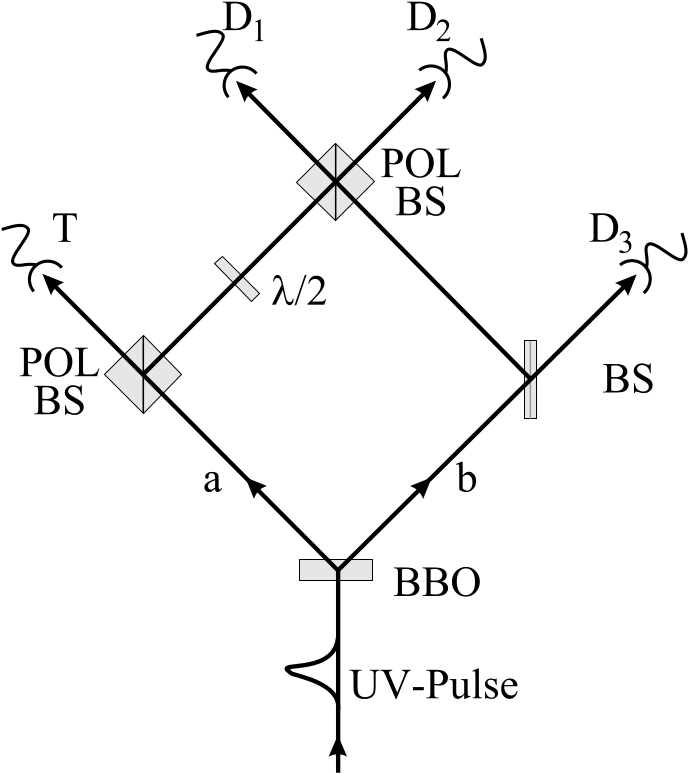
\includegraphics[width=0.4\textwidth]{Mainmatter/Chapter3/ghz-entanglement.png}
  \caption{Experimental set-up for GHZ entanglement demonstration.}
  \label{fig:ghz-entanglement}
\end{figure}

We begin this section by exposing a method that can be used to obtain systems of three particles exhibiting GHZ entanglement \cite{PhysRevLett.82.1345}.

Consider the experimental apparatus schematized in Fig. \ref{fig:ghz-entanglement}. Short pulses of ultraviolet light, which passes through a nonlinear crystal, generate pairs of polarization entangled photons in the state:
\begin{equation}
  \frac{1}{\sqrt{2}} \left( |H\rangle_a |V\rangle_b - |V\rangle_a |H\rangle_b \right),
\end{equation}
where the state $|H\rangle_a |V\rangle_b$ indicates a horizontally polarized photon in arm $a$ and a vertically polarized photon in arm $b$, conversely, the state $|V\rangle_a |H\rangle_b$ indicates a vertically polarized photon in arm $a$ and a horizontally polarized photon in arm $b$.

Continuing along arm $a$ we find a polarizing beam splitter that reflects vertically polarized photons and transmits horizontally polarized photons towards detector $T$. Reflected (vertically polarized) photons go then through a $\lambda/2$ plate that rotates polarization to $45^\circ$, then to a second polarizing beam splitter (analogous to the one already encountered) and finally to detectors $D_1$ ($V$ polarized photons) and $D_2$ ($H$ polarized photons).

Along arm $b$ we find a $50/50$ (polarization independent) beam splitter; transmitted photons go to detector $D_3$ while reflected photons go the second polarizing beam splitter of arm $a$ and finally to detectors $D_1$ ($H$ photons) and $D_2$ ($V$ photons).

All detectors, are behind narrow interference filters, the reason of which will be clarified later.

We want to show here that if two pairs are generated by a single pulse and each of the four photons is detected by one of the detectors $T$, $D_1$, $D_2$ and $D_3$ (exactly one photon per detector) then (with an additional hypothesis we will present in due time) a three photon GHZ state is recorded by detectors $D_1$, $D_2$ and $D_3$. Here is the reasoning: When such a fourfold detection is observed one photon in arm $a$ must have been $H$ polarized. Its companion in arm $b$, $V$ polarized, is either transmitted by the (non polarizing) beam splitter and detected by $D_3$ or reflected and detected by $D_2$ (each possibility with $50 \%$ chance). Consider the former case. Then the other photon in arm $b$, that must be $H$ polarized, is detected by $D_1$ and the last photon, coming through arm $a$, is detected by $D_2$ and is thus $H$ polarized. This situation corresponds to the detection of the state:
\begin{equation}
  |H\rangle_1 |H\rangle_2 |V\rangle_3
  \label{eq:hhv-state}
\end{equation}
by detectors $D_1$, $D_2$ and $D_3$. In the latter case an analogous argument leads us to conclude that the situation corresponds to the detection of the state:
\begin{equation}
  |V\rangle_1 |V\rangle_2 |H\rangle_3.
  \label{eq:vvh-state}
\end{equation}
The two possible states, (\ref{eq:hhv-state}) and (\ref{eq:vvh-state}), that correspond to a fourfold detection will not in general superpose coherently, thus will not give a GHZ state.

The statement we make now is that the lack of coherence is due to the possibility of obtaining information on the pair to which each photon belongs. If we can erase such information then a coherent superposition of the states (\ref{eq:hhv-state}) and (\ref{eq:vvh-state}) will be observed. Let us see why. When a single pulse generates a double pair, these come out from the source in the product state:
\begin{equation}
  \frac{1}{2} \left( |H\rangle_a |V\rangle_b - |V\rangle_a |H\rangle_b \right) \left( |H\rangle'_a |V\rangle'_b - |V\rangle'_a |H\rangle'_b \right).
  \label{eq:double-dc-state}
\end{equation}
The evolution of single components from the source to the detectors $T$, $D_1$, $D_2$ and $D_3$ is given by:
\begin{equation}
  \begin{split}
    |H\rangle_a &\rightarrow |H\rangle_T,\\
    |V\rangle_b &\rightarrow \frac{1}{\sqrt{2}} \left( |V\rangle_2 + |V\rangle_3 \right),\\
    |V\rangle_a &\rightarrow \frac{1}{\sqrt{2}} \left( |V\rangle_1 + |H\rangle_2 \right),\\
    |H\rangle_b &\rightarrow \frac{1}{\sqrt{2}} \left( |H\rangle_1 + |H\rangle_3 \right),
  \end{split}
  \label{eq:single-components-evolution}
\end{equation}
the same holds for the primed states. Substituting these expressions into (\ref{eq:double-dc-state}) and dropping the terms that do not correspond to fourfold detection we obtain, after normalization:
\begin{equation*}
    \frac{1}{2} \left( |H\rangle_T \left( |H\rangle'_1 |H\rangle'_2 |V\rangle_3 + |V\rangle'_1 |V\rangle_2 |H\rangle'_3 \right) + |H\rangle'_T \left( |H\rangle_1 |H\rangle_2 |V\rangle'_3 + |V\rangle_1 |V\rangle'_2 |H\rangle_3 \right) \right)
\end{equation*}
Finally, assuming that primed and unprimed photons are indistinguishable we obtain the state:%is some better comment needed here?
\begin{equation}
  \frac{1}{\sqrt{2}} |H\rangle_T \left( |H\rangle_1 |H\rangle_2 |V\rangle_3 + |V\rangle_1 |V\rangle_2 |H\rangle_3 \right).
  \label{eq:trigger+hv-ghz-state}
\end{equation}

In the experiment considered primed and unprimed photons could, in principle, be distinguished by measuring their energy (the four photon could all have different energies and the sum of the energies of the photons in each pair must be the same for both pairs) and by measuring the delay with which the photons are detected. As an example of this consider the case in which $T$ and $D_3$ fire simultaneously and $D_1$ and $D_2$ also fire simultaneously, this corresponds to one pair being detected by $T$ and $D_3$ and the other pair by $D_1$ and $D_2$. However, if the pulse that generates the two pairs is short and the interference filters behind which the photons are detected have a narrow bandwidth, such possibility of distinction is lost due to the spreading in time of the wave packets. The possibility of distinction by energy measurement is also lost because of the filters.

Experimental demonstration of GHZ entanglement obtained by means of the procedure just presented is reported in the same letter \cite{PhysRevLett.82.1345} which we summarize here.%could be better worded

\begin{figure}
  \centering
  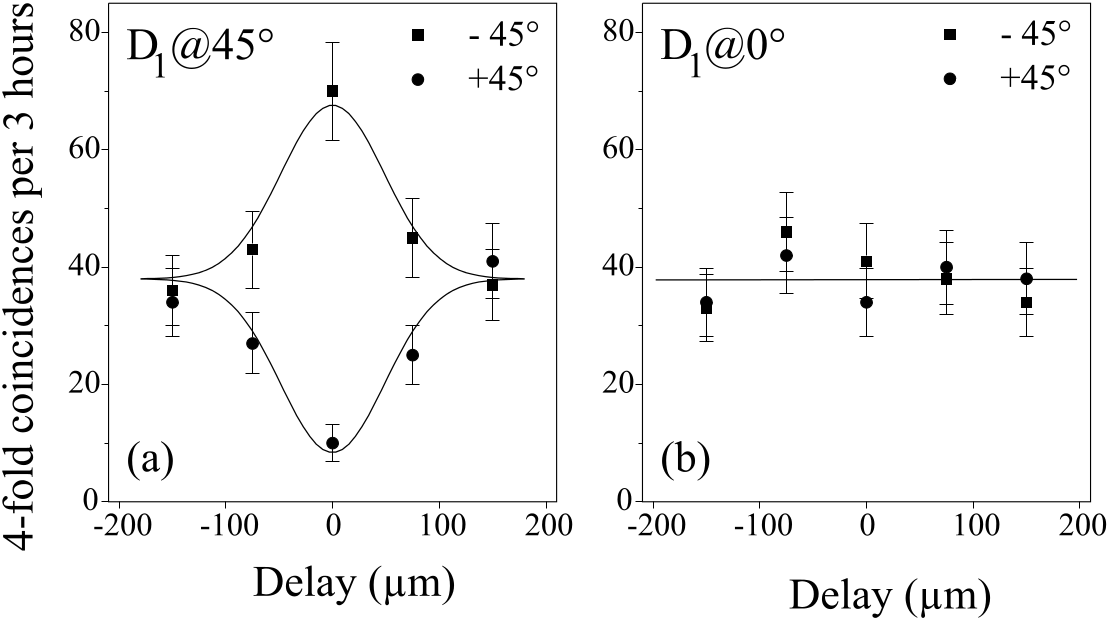
\includegraphics[width=0.6\textwidth]{Mainmatter/Chapter3/ghz-entanglement-exp-proof.png}
  \caption{``Experimental confirmation of GHZ entanglement. Graph (a) shows the results obtained for polarization analysis of the photon at $D_3$, conditioned on the trigger, and the detection of one photon at $D_1$ polarized at $+ 45^\circ$ and one photon at $D_2$ polarized at $- 45^\circ$. The two curves show the fourfold coincidences for a polarizer oriented at $+ 45^\circ$ and $- 45^\circ$, respectively, in front of detector $D_3$ as a function of the spatial delay in path $a$. The difference between the two curves at zero delay confirms the GHZ entanglement. By comparison [graph (b)] no such intensity difference is predicted if the polarizer in front of the detector $D_1$ is set at $0^\circ$.'' \cite{PhysRevLett.82.1345}}
  \label{fig:ghz-entanglement-exp-proof}
\end{figure}

First of all it is demonstrated that only the two components (\ref{eq:hhv-state}) and (\ref{eq:vvh-state}) are observed. This is done by comparison of the count rates of the eight possible combinations of polarization measurements ($H_1 H_2 H_3$, $H_1 H_2 V_3$, ..., $V_1 V_2 V_3$). A ratio $12:1$ between the expected and unexpected counts is reported. Second, it is demonstrated that the two components (\ref{eq:hhv-state}) and (\ref{eq:vvh-state}) form a coherent superposition (and not a statistical mixture). This is done by measuring the linear polarization of the photon detected by $D_1$ along the $+ 45^\circ$ bisector between the $H$ and $V$ directions. It is easy to show that such a measurement projects the state (\ref{eq:trigger+hv-ghz-state}) into:
\begin{equation*}
  \frac{1}{\sqrt{2}} |H\rangle_T |+ 45^\circ\rangle_1 \left( |H\rangle_2 |V\rangle_3 + |V\rangle_2 |H\rangle_3 \right),
\end{equation*}
that takes the following form when written on the $( |+ 45^\circ\rangle_i, |- 45^\circ\rangle_i), i = 2, 3$ basis:
\begin{equation*}
  \frac{1}{\sqrt{2}} |H\rangle_T |+ 45^\circ\rangle_1 \left( |+ 45^\circ\rangle_2 |+ 45^\circ\rangle_3 - |- 45^\circ\rangle_2 |- 45^\circ\rangle_3 \right).
\end{equation*}
The terms involving $|+ 45^\circ\rangle_2 |- 45^\circ\rangle_3$ and $|- 45^\circ\rangle_2 |+ 45^\circ\rangle_3$ interfere destructively, thus their absence indicates the coherent superposition of terms in (\ref{eq:trigger+hv-ghz-state}).

To show that it is the ``which-path'' information that destroys coherence measures at different delays are taken. This is obtained by varying path $a$ (and thus gradually restoring the possibility of pair distinction).

Fig. \ref{fig:ghz-entanglement-exp-proof} reports experimental results regarding the polarization of photon 3 for fourfold events in which photon 1 and 2 are polarized at $+ 45^\circ$ and $- 45^\circ$ respectively. Squares refer to $- 45^\circ$ polarization and circles to $+ 45^\circ$ polarization.

\begin{observation}
  The argument presented above and the subsequent experimental demonstration show that entanglement doesn't necessarily arise from interaction of the entangled subsystems. We want to give here a general illustration of such a fact taken from \cite{NYAS:NYAS91}.

Consider the factorized two particle state:
\begin{equation}
  |\psi\rangle = |\alpha\rangle_1 |\beta\rangle_2
  \label{eq:factorized-state}
\end{equation}
and the entangled state:
\begin{equation}
  |\Psi\rangle = \frac{1}{\sqrt{2}} \left( |a\rangle_1 |b\rangle_2 + |c\rangle_1 |d\rangle_2\right)
  \label{eq:entangled-state}
\end{equation}
where, for simplicity, $\langle a | c \rangle = \langle b | d \rangle = 0$.
Then, if (\ref{eq:factorized-state}) is not orthogonal to (\ref{eq:entangled-state}), it is possible to obtain an entangled state from (\ref{eq:factorized-state}) using the projection operator:
\begin{equation}
  P = |\Psi\rangle \langle\Psi|.
  \label{eq:projector}
\end{equation}

The experiment presented in this section can be seen as an actual realization of a projector of the type (\ref{eq:projector}). Another example of such a projector that has been experimentally realized is the one used in entanglement swapping experiments which is described in \cite{NYAS:NYAS91}.
\end{observation}

%\begin{observation}
%  ANALOGY WITH DOUBLE SLIT QUANTUM ERASER EXPERIMENT
%\end{observation}


\subsection{Claims regarding local-realism and quantum mechanics}
The experimental observations and analysis we have reported in the previous subsection are not sufficient to make statements against or in favor of local-realism (or quantum mechanics). For example the experimental procedure might be put into question because of the selection needed to isolate fourfold coincidences.

However it has been shown in \cite{PhysRevA.61.022109} that a more refined analysis of the experiment we have presented, together with some additional operational requirements, leads to the possibility of observing violations of local-realism (or of quantum mechanics). In fact claims of having observed such violations (of local-realism) have been made \cite{Nature.403.515}.

The matter of these two last references \cite{PhysRevA.61.022109} and \cite{Nature.403.515} is nevertheless beyond the scope of this thesis and will not be discussed further.

\begin{note}
  It is interesting to note the history of publication of references \cite{PhysRevLett.82.1345}, \cite{PhysRevA.61.022109} and \cite{Nature.403.515}.

  In reference \cite{PhysRevLett.82.1345} no claims regarding local-realism were made. Marek \.{Z}ukowski, informed of the results in \cite{PhysRevLett.82.1345}, carried out a more detailed analysis of the experiment. He found that minor adjustments were to be made in order to be in a position to make such claims \cite{PhysRevA.61.022109}. The same group of \cite{PhysRevLett.82.1345} published \cite{Nature.403.515} less than a month later than \cite{PhysRevA.61.022109}.
\end{note}

\chapter*{Conclusion}
\addcontentsline{toc}{chapter}{Conclusion}
In this thesis we have presented EPR's critique of quantum mechanics, we have seen that, under the assumptions of perfect correlation, reality and locality, quantum mechanics is not a complete description of reality (according to EPR's criterion of completeness).

We briefly mentioned the Bell's inequality, that can be derived from the EPR assumptions, and we have seen that the inequality is violated by statistical predictions of quantum mechanics.

Then we have illustrated the GHZ argument showing that the EPR reasoning doesn't apply to systems of three particles. We have seen that for such systems the EPR premises are inconsistent and, in contrast with Bell's argument, the contradiction arises for perfect correlations predicted by quantum mechanics\footnote{In \cite{:/content/aapt/journal/ajp/58/12/10.1119/1.16243} the authors note: ``There is an irony in this result in that perfect correlations are central to EPR's argument for the existence of states more complete than those of quantum mechanics.''}. Hence, the demonstration of the conflict between EPR's assumptions and quantum mechanics doesn't involve inequalities.

In the last chapter we have seen that, in principle, the GHZ reasoning allows to design experiments in which a single run (of the experiment) is sufficient to perform a test of quantum mechanics against local-realism. To our knowledge no experiment of this type has been performed.

Finally, we have discussed some actual experimental effort towards a test of quantum mechanics following the GHZ argument. We have presented an experiment that has been performed to observe GHZ entanglement, but the analysis we have reported didn't allow us to make claims in favor or against quantum mechanics. However, we have given reference to a more refined analysis of a slightly modified version of the experiment that allowed such claims to be made.

The techniques employed in the experiment we have presented also allowed us to observe that entanglement doesn't necessarily arise from interaction of the entangled subsystems but can also be obtained by a suitable projection (onto an entangled state) of a factorized state.


\appendix
\chapter[Appendix]{}
\label{app:spin-predictions}

\section{Singlet state representation on different bases}
We prove here that the state of equation (\ref{eq:singlet-state}) takes the same form on all orthonormal bases of the $S_x$, $S_y$ and $S_z$ observables.

Let us prove that the state:
\begin{equation}
  |\chi\rangle_{\mathbf{\hat{z}}} = \frac{1}{\sqrt{2}} \left( |\mathbf{\hat{z}}, +\rangle_1 |\mathbf{\hat{z}}, -\rangle_2 - |\mathbf{\hat{z}}, -\rangle_1 |\mathbf{\hat{z}}, +\rangle_2 \right)
  \label{eq-singlet-state-z}
\end{equation}
has the same form on the tensor basis obtained from the two bases $\left( |\mathbf{\hat{x}}, +\rangle_i, |\mathbf{\hat{x}}, -\rangle_i \right), i = 1, 2$ the same argument can be adapted to the $\mathbf{\hat{y}}$ case.

Let us write the $S_x$ operator as a $2 \times 2$ matrix on the $\left( |\mathbf{\hat{z}}, +\rangle_i, |\mathbf{\hat{z}}, -\rangle_i \right)$ basis:
\begin{equation*}
  S_x =
  \begin{pmatrix}
    0 & 1\\
    1 & 0
  \end{pmatrix}
\end{equation*}
in units $\frac{\hbar}{2} = 1$. This operator can be diagonalized leading to the eigenvectors:
\begin{equation}
  \begin{split}
    |\mathbf{\hat{x}}, +\rangle_i &= \frac{1}{\sqrt{2}} \left( |\mathbf{\hat{z}}, +\rangle_i + |\mathbf{\hat{z}}, -\rangle_i \right),\\
    |\mathbf{\hat{x}}, -\rangle_i &= \frac{1}{\sqrt{2}} \left( |\mathbf{\hat{z}}, +\rangle_i - |\mathbf{\hat{z}}, -\rangle_i \right)
  \end{split}
  \label{eq:sx-eingenvectors}
\end{equation}
with eigenvalues $+ 1$ and $- 1$ respectively. Inverting the two equations (\ref{eq:sx-eingenvectors}) and substituting into (\ref{eq-singlet-state-z}) leads to the desired result.

\section{Quantum mechanical predictions on GHZ states}
We derive here the predictions of quantum mechanics of which we made use in Chapter \ref{chap:ghz-theorem}. Namely, we will show that the state of equation (\ref{eq:ghz-state}), i.e.:
\begin{equation*}
  |\chi\rangle = |+\rangle_1 |+\rangle_2 |+\rangle_3 - |-\rangle_1 |-\rangle_2 |-\rangle_3
\end{equation*}
is an eigenstate of all of the observables (\ref{eq:xyy-observables}), i.e.:
\begin{equation}
  \begin{split}
    S_{1x} \times S_{2y} \times S_{3y}\\
    S_{1y} \times S_{2x} \times S_{3y}\\
    S_{1y} \times S_{2y} \times S_{3x}
  \end{split}
  \label{eq:xyy-operators-app}
\end{equation}
with eigenvalue $+ 1$ and it is also eigenstate of the observable (\ref{eq:xxx-observable}), i.e.:
\begin{equation*}
  S_{x1} \times S_{2x} \times S_{3x}
\end{equation*}
this time with eigenvalue $- 1$.

Let us prove this statement for the first observable in (\ref{eq:xyy-operators-app}) the same argument can be adapted to the other observables. We begin with the spin of particle 1:
\begin{equation*}
  \begin{split}
    S_{1-} |\chi\rangle &= 2 |-\rangle_1 |+\rangle_2 |+\rangle_3\\
    S_{1+} |\chi\rangle &= - 2 |+\rangle_1 |-\rangle_2 |-\rangle_3
  \end{split}
\end{equation*}
that gives:
\begin{equation*}
  |\chi\rangle' := S_{1x} |\chi\rangle = |-\rangle_1 |+\rangle_2 |+\rangle_3 - |+\rangle_1 |-\rangle_2 |-\rangle_3.
\end{equation*}
For particle 2 we have:
\begin{equation*}
  \begin{split}
    S_{2-} |\chi\rangle' &= 2 |-\rangle_1 |-\rangle_2 |+\rangle_3\\
    S_{2+} |\chi\rangle' &= - 2 |+\rangle_1 |+\rangle_2 |-\rangle_3
  \end{split}
\end{equation*}
thus:
\begin{equation*}
  |\chi\rangle'' := S_{2y} |\chi\rangle' = - \frac{1}{i} |+\rangle_1 |+\rangle_2 |-\rangle_3 + |-\rangle_1 |-\rangle_2 |+\rangle_3.
\end{equation*}
The same goes through for particle 3 and leads to:
\begin{equation*}
  |\chi\rangle''' := S_{3y} |\chi\rangle'' = |+\rangle_1 |+\rangle_2 |+\rangle_3 - |-\rangle_1 |-\rangle_2 |-\rangle_3 = |\chi\rangle.
\end{equation*}
which is the desired result.


%backmatter

%\begin{singlespace}
\bibliography{Backmatter/bibliography}
\bibliographystyle{unsrt}
%\end{singlespace}


\end{document}
